\documentclass[12pt]{article}
\usepackage[utf8]{inputenc}

%THIS IS WHERE ALL THE SYDE STUFF IS
\usepackage{sydestyle}

% Other imports go here
\usepackage{graphicx}
\graphicspath{{figures/}}
\usepackage{notoccite}

% Fill in this blob

\title{Design of a Latex WTR Following the SYDE Guide}
\author{Erik Derohanian}
\studentnumber{12345678}
\lastsemester{3A}
\date{January 12, 1978}
\employer{Gandalf Technologies}
\employeraddress{130 Colonnade Road \\ Nepean, ON K2E 1B6}



% Content here
\begin{document}
	% Specify start indent because other wise it may not line up perfectly with the default
	% indents when we use the indent shortcuts
	\startindent
	% Start with a title page!
	\makewtrtitle

	% Your letter of submittal should go here, and it's not indented
	\stopindent
        \begin{spacing}{1.0}

	YOUR RETURN ADDRESS HERE \\

    	September 32, 1984 \\

    	Dr. FILL ME IN, Professor and Chair, \\
    	Department of Systems Design Engineering, University of Waterloo \\
    	Waterloo, Ontario, Canada \\
    	N2L 3G1\\
    	
    	Dear Prof. FILL ME IN, \\
    
        I have prepared this report, “Design of a Latex WTR Following the SYDE Guide,” as my 3B Work Report for the Engineering team at Gandalf Technologies. This report is the FIRST SECOND FINAL of three that I must submit as part of my degree requirements, and it has not received any previous academic credit. This report was entirely written by me and has not received any previous academic credit at this or any other institution.\\
    	
    	FILL ME IN Write some stuff about the company briefly, name your manager, etc. \\
    	
    	The purpose of this report is to ... FILL ME IN. Write a one or two sentence, VERY BRIEF overview of the report. \\

    	Sincerely,
    
    	\begin{figure}[!ht]
        
\includegraphics[width=0.15\textwidth]{signature}
        \end{figure}
    	
    	Erik Derohanian \\
    	12345678 \\
    	3B Systems Design Engineering

	\end{spacing}
	% new page at the end of the letter and resume indenting
	\newpage
	\startindent

	% Abstract
	\begin{abstract}
		This is a \LaTeX\ style that aims to match the uWaterloo SYDE style guide because doing work term report formatting makes me want to ahkerfg kasjrgu dfhgukia rgfzjkxfh aeguxdfgzxyu auisdrjgfh ifawuiegf isdurgfia uewrzcjbn zkjdfcvmba weukirydfui erjk t  zxcg awr sdfh stry sdfh yukstrh f nynyuikjef acse fcvdt ukyivegt hac erctse rgc.
	\end{abstract}

	% Make a table of contents.
	\addcontentsline{toc}{section}{Table of Contents}
	\tableofcontents
	\newpage

	% List of figures and tables.
	\addcontentsline{toc}{section}{List of Figures}
	\listoffigures
	\newpage
	\addcontentsline{toc}{section}{List of Tables}
	\listoftables
	\newpage

	% Couldn't figure out how to automate this, but leave this line in to restart page numbers at 1 and with arabic numbers.
	\startarabicpagenumbers

	\section{First section}

	Your text goes here. I'm going to add a bunch of words to make this a paragraph longer than one line.

	The next paragraph is automatically indented, as per the guide (default \LaTeX\ behaviour)

	\subsection{A subsection}

	More text.

	\subsubsection{A sub-subsection}

	Yep, it's actually a \textbackslash subsubsection\{sub-subsection name\}.

	\section{Some Tables and Figures}

	Here is a figure:

	\begin{figure}[!ht]
	\centering
	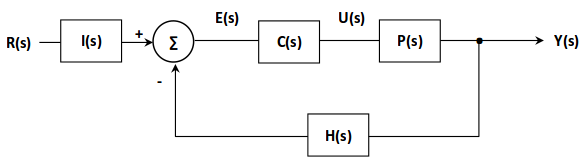
\includegraphics[width=0.7\textwidth]{pcontroller}
	\caption{System diagram of a P controller}
	\label{pcontroller}
	\end{figure}

	I can start talking about that figure, and refer to it as figure \ref{pcontroller} and the number will update based on the label which is very useful when you're shuffling stuff around because you don't have to keep track of figure numbers.

	We can also do tables, like so

	\begin{center}
		\begin{table}[!ht]
			\caption{Some table I copied from the Latex wikibook online}
			\begin{tabular}{ | l | l | l | p{5cm} |}
			\hline
			Day & Min Temp & Max Temp & Summary \\ \hline
			Monday & 11C & 22C & A clear day. \\ 	\hline
			Tuesday & 9C & 19C & Cloudy with rain.\\ \hline
			Wednesday & 10C & 21C & Rain. \\
			\hline
			\end{tabular}
			\label{shittytable}
		\end{table}
	\end{center}

	Like the previous figure, we can refer to this table as table \ref{shittytable}.

	Here is a kitten:

	\begin{figure}[!ht]
	\label{kitten}
	\centering
	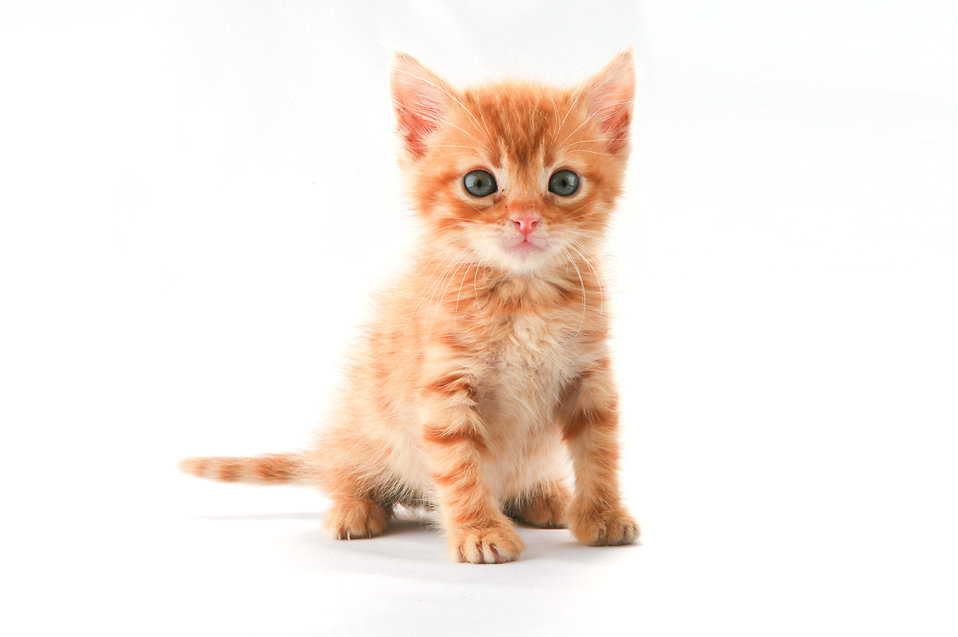
\includegraphics[width=0.5\textwidth]{kitten}
	\caption{It's a kitten. You like kittens.}
	\end{figure}

	\section{Equations}

	Here is the transfer function to the control system shown in figure \ref{pcontroller}:

	\begin{equation}
	\label{ptransfer}
	T(s)=\frac{Y(s)}{R(s)}=I(s) \cdot \frac{K_p \cdot P(s)}{1 + K_p \cdot P(s) \cdot H(s)}
	\end{equation}

	As usual, we can use it's number. That was formula \eqref{ptransfer}

	\section{Citations}

	Three items are cited: \textit{The \LaTeX\ Companion} book \cite{latexcompanion}, the Einstein journal paper \cite{einstein}, and the Donald Knuth's website \cite{knuthwebsite}. The \LaTeX\ related items are \cite{latexcompanion,knuthwebsite}.

	\newpage
	\startappendixtitles
	\begin{appendices}

	\section{Glossary}
	% In the specific case of a glossary, you probably don't want to indent every new definition
	\stopindent
	word: some def

	word2: some other def

	\startindent
	\end{appendices}
	\finishappendixtitles

	\makesydebib{references}

\end{document}
